\documentclass[a4paper, 10pt]{article}

\usepackage[utf8]{inputenc}
\usepackage[spanish]{babel}
\usepackage{graphicx}
\usepackage{geometry}
\usepackage{listings}
\usepackage{amsmath}
\usepackage{amsfonts}
\usepackage{amssymb}
\usepackage{caratula}
\usepackage[section]{placeins}
\usepackage{titlesec}

\newcommand{\Z}{\mathbb{Z}}
\def\code#1{\texttt{#1}}
\newcommand\tab[1][0.5cm]{\hspace*{#1}}

\geometry{a4paper, margin=0.7in}

\begin{document}
    %Caratula
    \pagenumbering{gobble}
    \newpage

    \begin{center}
        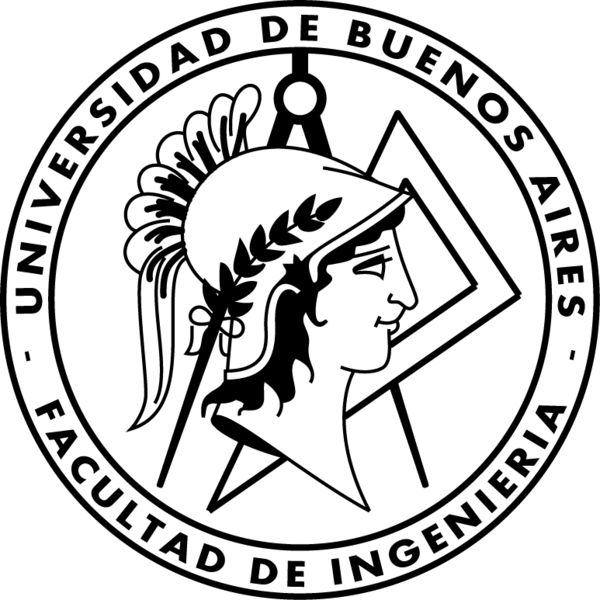
\includegraphics[width=7.5cm, height=7.5cm]{images/logo}
    \end{center}

    \materia{Organización de Datos}
    \submateria{Segundo Cuatrimestre 2017}
    \titulo{Trabajo Práctico 1}

    \integrante{Rodrigo De Rosa}{97799}{rodrigoderosa@outlook.com}
    \integrante{Marcos Schapira}{97934}{schapiramarcos@gmail.com}
    \integrante{Facundo Guerrero}{97981}{facundoiguerrero@gmail.com}
    \maketitle
    %Fin caratula
    %Table of contents
    \newpage
    \pagenumbering{roman}
    \tableofcontents
    %Fin table of contents
    %Informe
    \newpage
	\pagenumbering{arabic}
	\part{Análisis del tipo de las propiedades}
		En esta parte, se analizará como las distintas características de las propiedades son afectadas por el tipo de propiedad.
		Esto es, si son negocios, casas, PHs o departamentos.
		\section{Tipos de propiedades y sus superficies}
			La idea de esta sección es analizar en que lugares podemos encontrar a las propiedades con mayor y menor superficie
			en CABA y GBA.
			\subsection{¿Dónde están las propiedades más grandes según su tipo?}
				\subsubsection{Casas}
				\subsubsection{PHs}
				\subsubsection{Departamentos}
				\subsubsection{Locales}
			\subsection{¿Dónde están las propiedades más chicas según su tipo?}
				%Bottom 5				
				\subsubsection{Casas}
				\subsubsection{PHs}
				\subsubsection{Departamentos}
				\subsubsection{Locales}
		\section{Tipos de propiedades y sus precios}
			\subsection{¿Dónde están las propiedades más caras según su tipo?}
				%Top 5				
				\subsubsection{Casas}
				\subsubsection{PHs}
				\subsubsection{Departamentos}
				\subsubsection{Locales}
			\subsection{¿Dónde están las propiedades más baratas según su tipo?}
				%Bottom 5				
				\subsubsection{Casas}
				\subsubsection{PHs}
				\subsubsection{Departamentos}
				\subsubsection{Locales}
		\section{Tipos de propiedades y sus ubicaciones}
			\subsection{¿En qué lugar hay más propiedades de cada tipo?}
				%Top 5 (heat-map)
				\subsubsection{Casas}
				\subsubsection{PHs}
				\subsubsection{Departamentos}
				\subsubsection{Locales}
		\section{Variación del precio total a través de los años}
			\subsection{Casas}
			\subsection{PHs}
			\subsection{Departamentos}
			\subsection{Locales}
		\section{Variación del precio por $m^2$ a través de los años}
			En esta sección, el objetivo es analizar la variación del precio por $m^2$ de cada uno de los tipos de propiedad
			disponibles. Se espera que, en todos los casos, la variación sea creciente alcanzando su máximo en 2017. De todas formas,
			el objetivo es ver cuál varió más y cómo fue dicha variación.
			\subsection{¿Cuál fue el tipo de propiedad más caro en cada año?}
				En este caso, la pregunta es: año a año, cuál fue el tipo de propiedad con mayor precio por $m^2$.
				\subsubsection{2013}
					Para el año 2013, podemos ver que los departamentos fueron los más caros, teniendo en segundo lugar a los
					PHs, en tercero a las casas y finalmente a los locales.
					\begin{center}
   		    				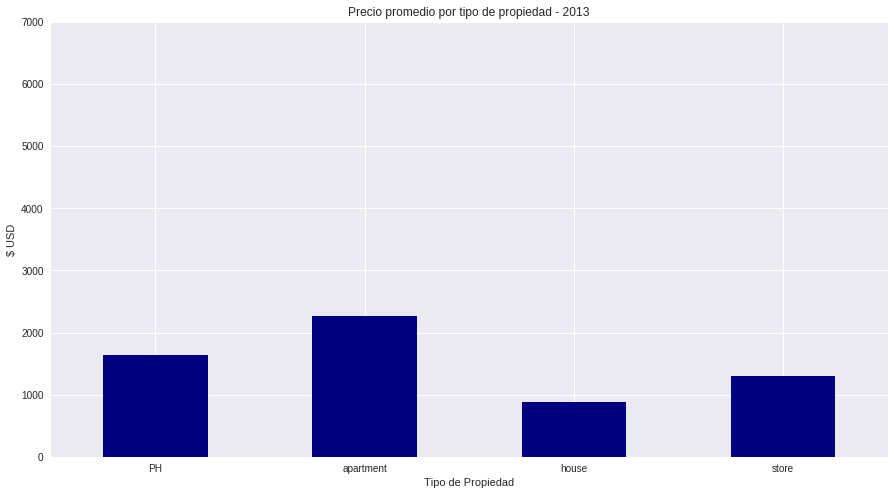
\includegraphics[width=\textwidth]{images/propPrice2013}
				  	\end{center}
				\subsubsection{2014}
					En 2014 se observa un aumento en los precios de los locales mientras que el resto de los tipos de propiedad
					se mantienen casi igual.
					\begin{center}
   		    				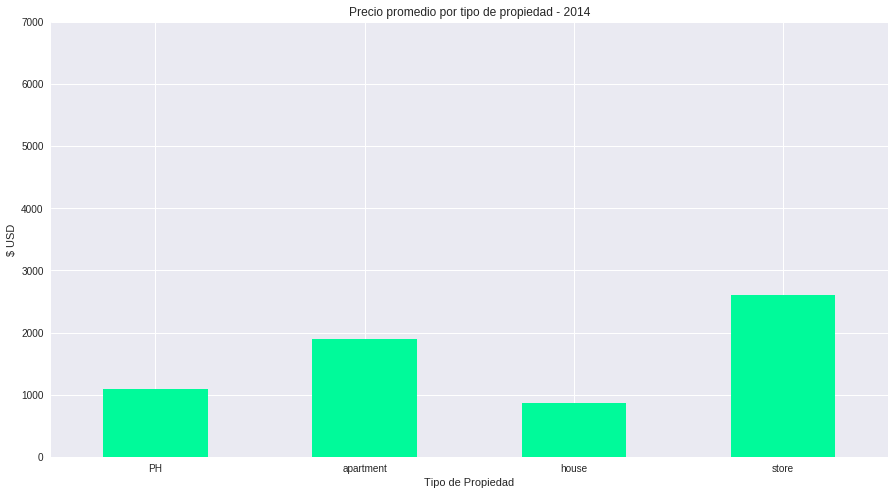
\includegraphics[width=\textwidth]{images/propPrice2014}
				  	\end{center}
				\subsubsection{2015}
					Ahora, en el año 2015, podemos ver que la forma es igual que en 2014 aunque con precios levemente más elevados.
					\begin{center}
   		    				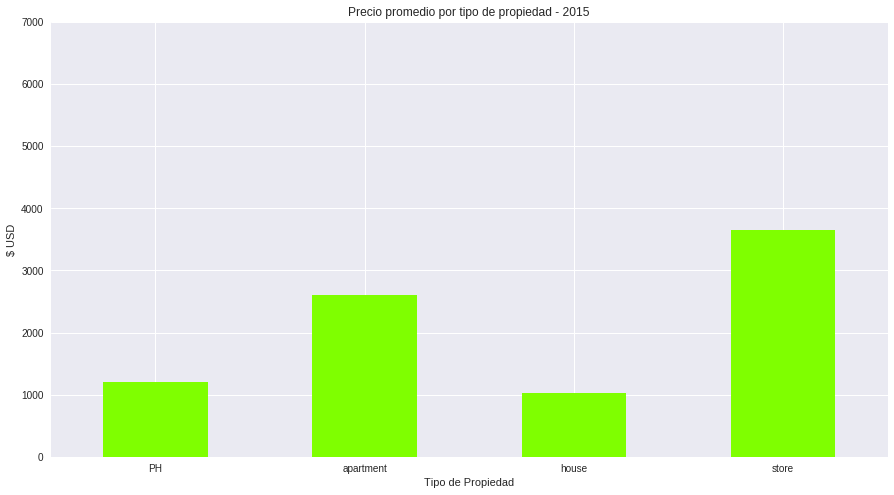
\includegraphics[width=\textwidth]{images/propPrice2015}
				  	\end{center}
				\subsubsection{2016}
					Para 2016 se encuentra una suba en los precios en general y un ascenso al segundo puesto de los PHs, mientras
					que los locales siguen en el primer puesto.
					\begin{center}
   		    				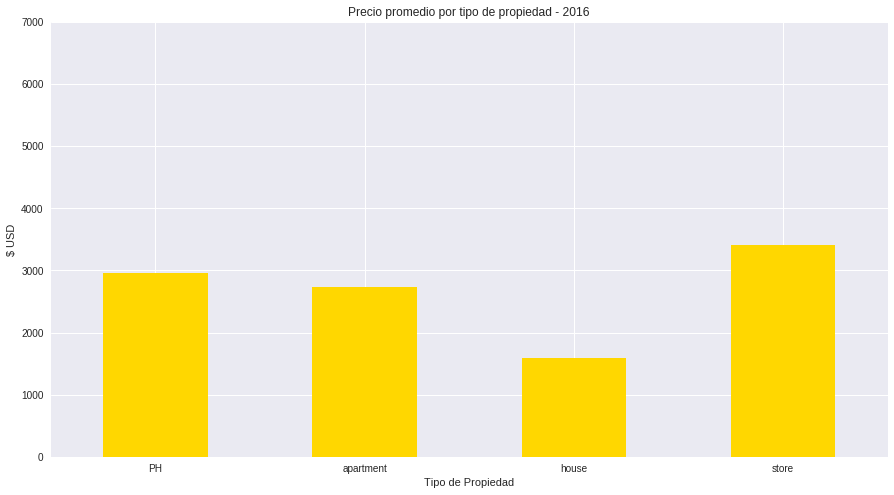
\includegraphics[width=\textwidth]{images/propPrice2016}
				  	\end{center}
				\subsubsection{2017}
					Finalmente, en 2017 vuelven a tomar el segundo puesto los departamentos y se ve el aumento más grande en los
					cuatro años, llegando los locales a un promedio de $7000$USD.
					\begin{center}
   		    				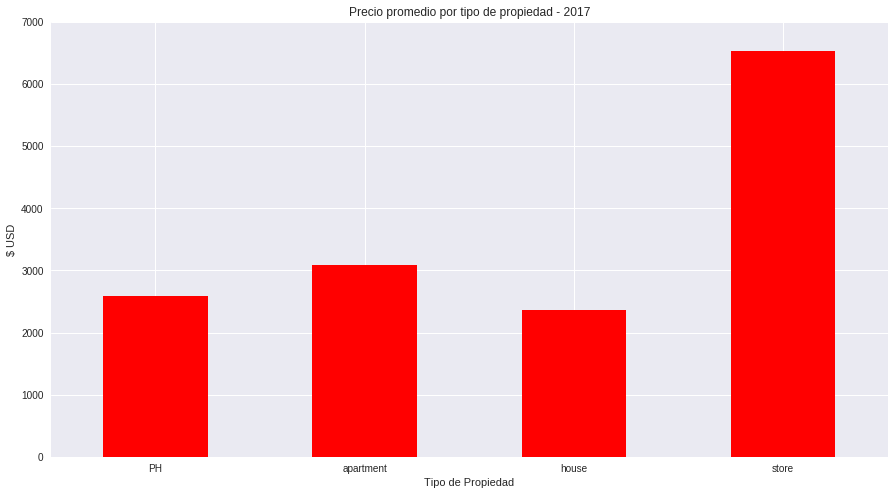
\includegraphics[width=\textwidth]{images/propPrice2017}
				  	\end{center}
			\subsection{Casas}
				En el caso de las casas nos encontramos con una variación muy pequeña para el intervalo $[2013, 2015]$ y mucho
				más marcada para los últimos dos años. De todos modos, en total, la variación es de aproximadamente $1500$USD.
				\begin{center}
   		    			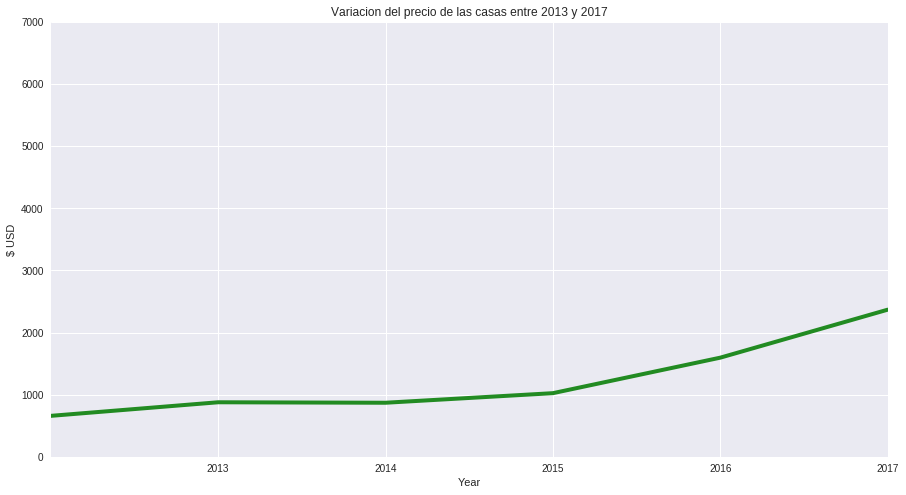
\includegraphics[width=\textwidth]{images/houseVariation}
				\end{center}
			\subsection{PHs}
				En este caso, si bien la variación es de aproximadamente $1000$USD, vemos que en el año 2015 hubo un aumento del
				valor de los PHs de aproximadamente $2000$USD, con un posterior decrecimiento durante 2016 y 2017. Este tipo
				de propiedad tuvo descensos y ascensos alternados, uno cada año.
				\begin{center}
   		    			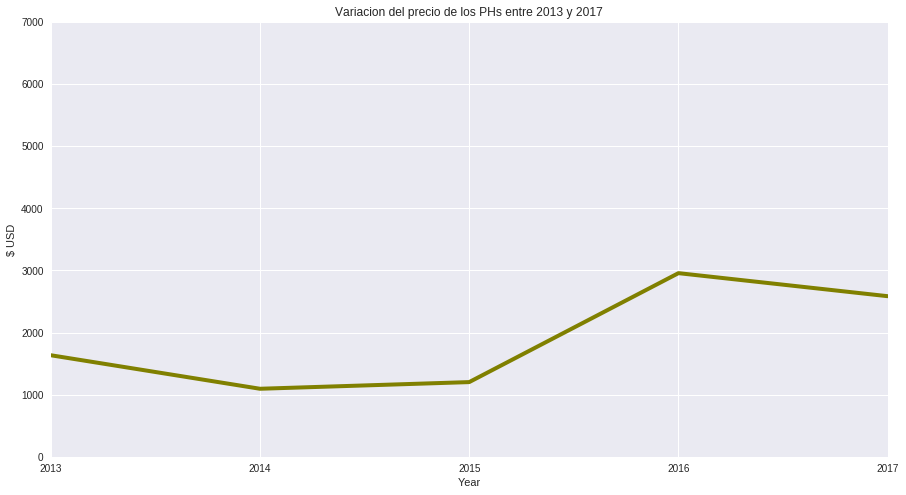
\includegraphics[width=\textwidth]{images/phVariation}
				\end{center}
			\subsection{Departamentos}
				Nuevamente encontramos un aumento de aproximadamente $1000$USD en el valor de los departamentos entre los cuatro
				años, con un descenso entre 2013 y 2014 pero con un aumento en los años siguientes.
				\begin{center}
   		    			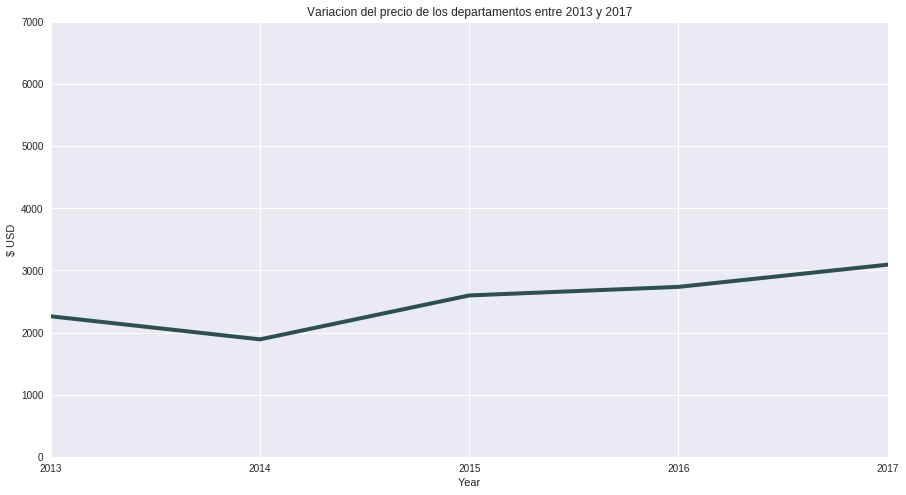
\includegraphics[width=\textwidth]{images/apartmentsVariation}
				\end{center}
			\subsection{Locales}
				Finalmente, en el caso de los locales, podemos ver que el aumento es exageradamente grande (aproximadamente del
				$600\%$) en el paso de los últimos cuatro años. Se puede observar un aumento con una gran pendiente en los primeros
				dos años, un leve descenso entre 2015 y 2016 y finalmente un nuevo aumento importante. \\
				\tab Consideramos que la magnitud de esta variación se puede deber a dos cosas; la primera es que efectivamente los
				precios por $m^2$ de los locales haya aumentado de esta manera y la segunda es que los numeros obtenidos se deban
				a la poca cantidad de entradas que se poseen de los primeros tres años. De todas maneras, reforzando la primer 
				opción, el año 2016 y 2017 poseen una cantidad de entradas muy similar y el cambio es de unos $3000$USD.
				\begin{center}
   		    			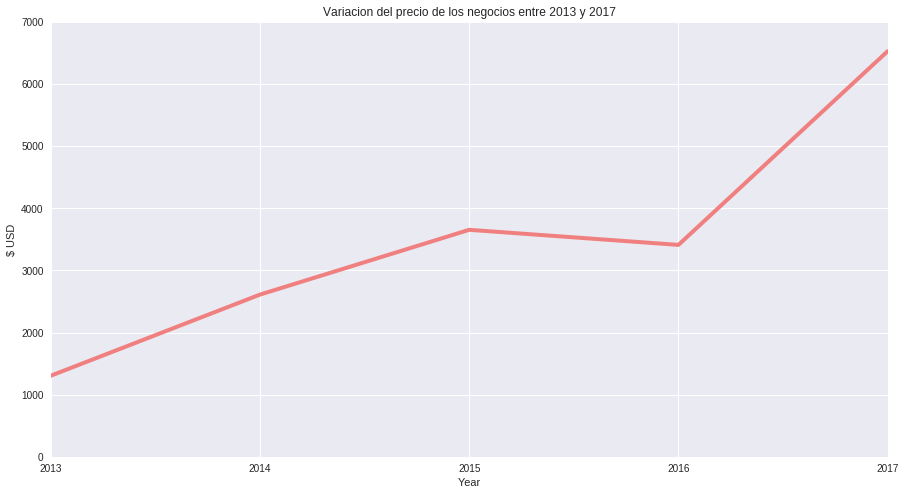
\includegraphics[width=\textwidth]{images/storeVariation}
				\end{center}
			\subsection{Análisis conjunto}
				Por último, uniremos los previos cuatro gráficos para un análisis conjunto de los datos obtenidos.
				\begin{center}
   		    			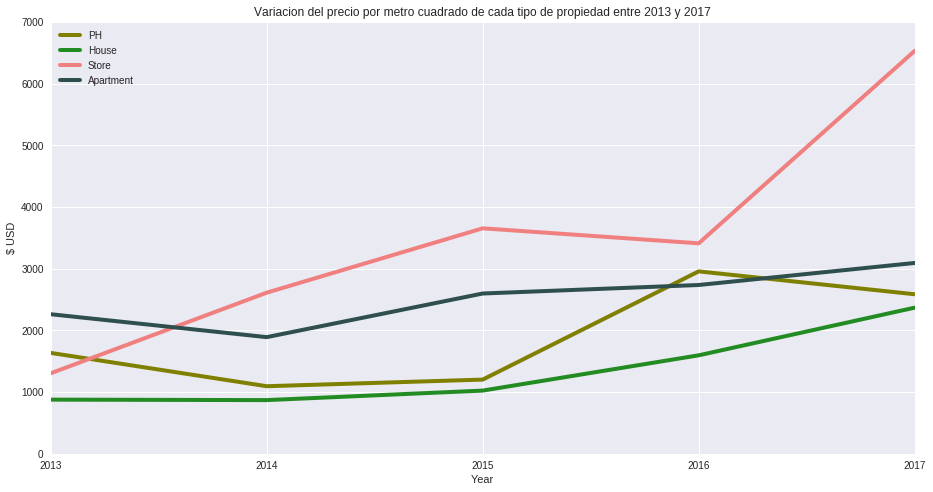
\includegraphics[width=\textwidth]{images/jointVariation}
				\end{center}
				\tab Aquí se puede ver que todas las viviendas tienen una variación similar y que su precio en 2017 es muy similar.
				Por otro lado, los locales destacan por su bajo comienzo (casi último) y su alto final (primero con más de $3000$USD
				de diferencia). \\
				\tab Podemos concluír, entonces, notando que la relación de precios se mantuvo con el pasar de los años, manteniendo
				el orden de los precios. Es decir, los departamentos son los más caros, seguidos por los PHs y terminando con 
				las casas pero con precios cada vez mayores, como se esperaba.
		
\end{document}